% !TeX spellcheck = ru_RU
% !TEX root = vkr.tex

\section{Описание решения}
\label{sec:solution}

В рамках данной работы была реализована архитектура распределённого выполнения сетевых эмуляций в рамках проекта Miminet\cite{miminet} с использованием Docker и системы управления задачами Celery + RabbitMQ\cite{rabbitmq}.
Это позволило повысить масштабируемость платформы и сократить время ожидания запуска эмуляции для студентов.

\subsection{Разработка архитектуры распределённого выполнения эмуляций}
\label{subsec:task1}

Изначально все эмуляции в Miminet\cite{miminet} выполнялись в одном контейнере, что ограничивало масштабируемость: увеличение числа одновременных задач приводило к росту времени ожидания и перегрузке одного ядра CPU.

Предложенное решение включает запуск нескольких изолированных Docker-контейнеров, каждый из которых может выполнять одну или несколько эмуляций. Контейнеры работают независимо и получают задания из общей очереди RabbitMQ\cite{rabbitmq}, а изоляция каждой эмуляции реализована с помощью Mininet\cite{mininet}.

Каждый контейнер содержит воркер Celery\cite{celery}, получающий задачи из общей очереди. Такая схема позволяет масштабировать систему горизонтально — за счёт увеличения количества рабочих контейнеров без изменения основной логики.

\begin{figure}[H]
  \centering
  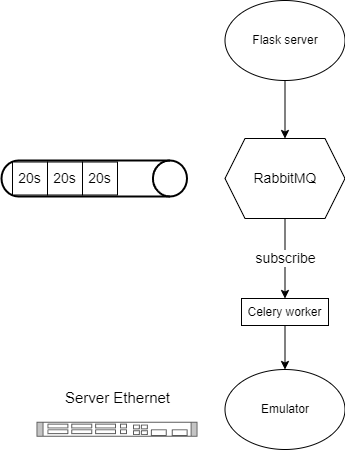
\includegraphics[width=0.40\textwidth]{figures/seq.png}
  \caption{Сравнение архитектур: исходная (один контейнер)}
  \label{fig:arch_compare}
\end{figure}

\begin{figure}[H]
  \centering
  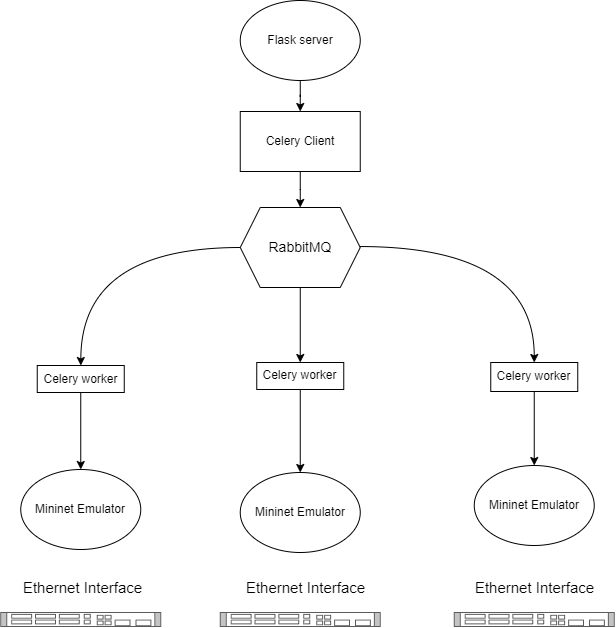
\includegraphics[width=0.60\textwidth]{figures/example.png}
  \caption{Сравнение архитектур: новая (множество контейнеров)}
  \label{fig:arch_compare}
\end{figure}

\subsection{Проектирование и внедрение системы управления задачами}
\label{subsec:task2}

Для распределения задач по контейнерам была использована связка Celery\cite{celery} + RabbitMQ\cite{miminet}.
Celery\cite{celery} позволяет организовать очередь заданий и обеспечивает параллельное выполнение с учётом текущей загрузки.

В рамках данной работы была выполнена:
\begin{itemize}
  \item настройка очереди заданий для передачи задач воркерам.
  \item параметризация контейнеров (например, через переменные окружения) для запуска с разными конфигурациями.
\end{itemize}

Каждый контейнер при старте подключается к общей очереди RabbitMQ\cite{rabbitmq} и ожидает задания.
Как только задача поступает — она исполняется и возвращает результат в центральную систему.

Такой подход позволяет эффективно масштабировать систему, добавляя или отключая контейнеры без необходимости остановки сервиса.

\subsection{Экспериментальное тестирование и валидация}
\label{subsec:task3}

Для проверки эффективности решения были проведены эксперименты с запуском 20 эмуляций в двух режимах:
\begin{itemize}
  \item один контейнер с одним воркером (исходная реализация Miminet);
  \item четыре контейнера, работающие параллельно (предложенная в рамках данной работы).
\end{itemize}

\subsubsection*{Методика}

В каждой эмуляции вручную фиксировалось время выполнения:

\begin{minted}[frame=single]{python}
import time
start = time.time()
# выполнение эмуляции
end = time.time()
print(f"Эмуляция завершена за {end - start:.2f} сек.")
\end{minted}

\subsubsection*{Метрики}
\begin{itemize}
  \item Общее время выполнения заданий.
  \item Средняя загрузка CPU.
  \item Среднее время ожидания запуска эмуляции для студентов сократилось.
  \item Количество одновременно исполняемых эмуляций.
\end{itemize}

\begin{table}[H]
\centering
\caption{Сравнение производительности}
\label{tab:cmp}
\begin{tabular}{|c|c|c|}
\hline
Конфигурация & Общее время (сек) & Ускорение \\
\hline
1 контейнер & 100 & 1.0$\times$ \\
4 контейнера & 25 & 4.0$\times$ \\
\hline
\end{tabular}
\end{table}

\begin{figure}[H]
  \centering
  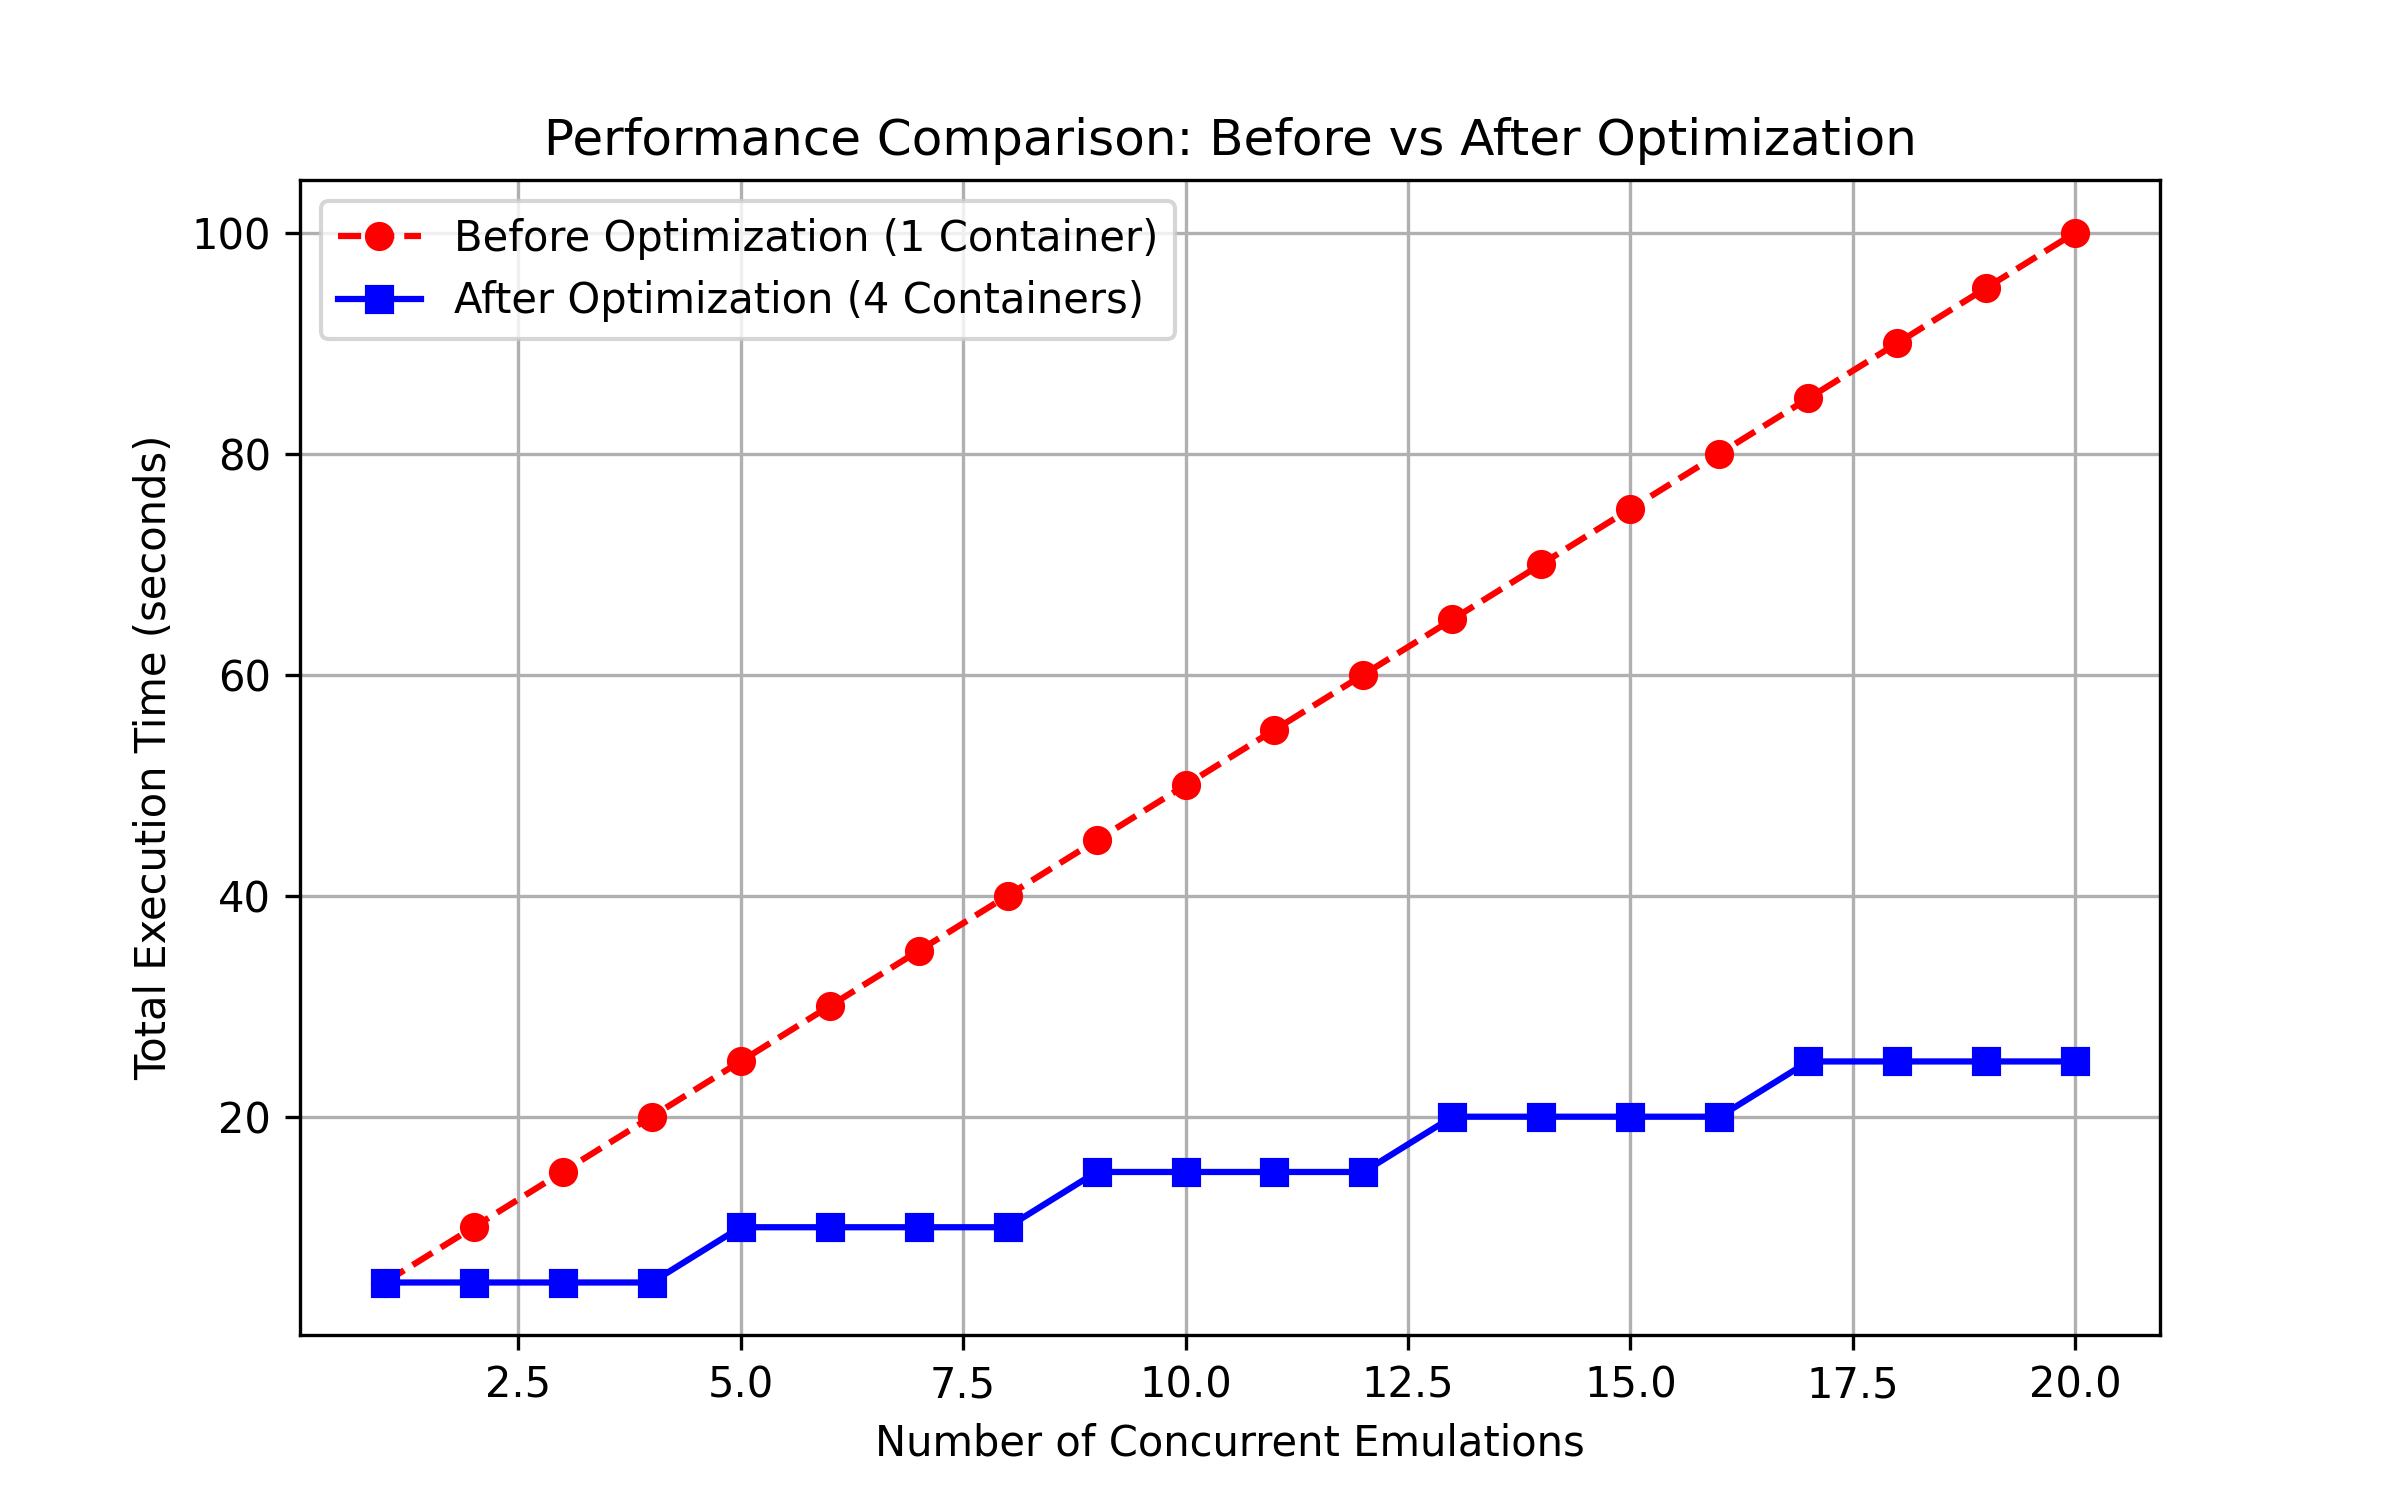
\includegraphics[width=0.75\textwidth]{figures/performance_comparison.png}
  \caption{График сравнения времени при запуске 20 эмуляций}
  \label{fig:perf}
\end{figure}

Эксперименты показали, что система с несколькими контейнерами позволяет запускать больше эмуляций одновременно и равномерно распределяет нагрузку между ядрами процессора.

Это, в свою очередь, приводит к сокращению времени ожидания и повышению эффективности обучения.

\textbf{Выводы:}
\begin{itemize}
  \item Количество параллельно исполняемых задач увеличилось в 4 раза;
  \item Загрузка CPU распределяется равномерно между ядрами;
  \item Среднее время ожидания студентом до начала эмуляции сокращается с 100 до 25 секунд.
\end{itemize}

\subsection{Итоги реализации}
\label{subsec:summary}

Предложенное решение было внедрено в существующий код проекта Miminet и протестировано в условиях, приближённых к реальному использованию студентами. Архитектура допускает дальнейшее масштабирование и автоматизацию (например, динамическое добавление контейнеров на основе текущей загрузки).

Исходный код решения доступен в открытом репозитории: \url{https://github.com/mimi-net/miminet}
